% 
% Annual Cognitive Science Conference
% Sample LaTeX Paper -- Proceedings Format
% 

% Original : Ashwin Ram (ashwin@cc.gatech.edu)       04/01/1994
% Modified : Johanna Moore (jmoore@cs.pitt.edu)      03/17/1995
% Modified : David Noelle (noelle@ucsd.edu)          03/15/1996
% Modified : Pat Langley (langley@cs.stanford.edu)   01/26/1997
% Latex2e corrections by Ramin Charles Nakisa        01/28/1997 
% Modified : Tina Eliassi-Rad (eliassi@cs.wisc.edu)  01/31/1998
% Modified : Trisha Yannuzzi (trisha@ircs.upenn.edu) 12/28/1999 (in process)
% Modified : Mary Ellen Foster (M.E.Foster@ed.ac.uk) 12/11/2000
% Modified : Ken Forbus                              01/23/2004
% Modified : Eli M. Silk (esilk@pitt.edu)            05/24/2005
% Modified : Niels Taatgen (taatgen@cmu.edu)         10/24/2006
% Modified : David Noelle (dnoelle@ucmerced.edu)     11/19/2014

%% Change "letterpaper" in the following line to "a4paper" if you must.

\documentclass[10pt,letterpaper]{article}

\usepackage{hyperref}
\usepackage{cogsci}
\usepackage{pslatex}
\usepackage{graphicx}
\usepackage{apacite}
\usepackage{color}

\definecolor{Red}{RGB}{255,0,0}
\newcommand{\red}[1]{\textcolor{Red}{#1}}

\newcommand{\jd}[1]{\green{$^*$}\marginpar{\footnotesize{JD: \green{#1}}}}

\newcommand{\subsubsubsection}[1]{{\em #1}}
\newcommand{\eref}[1]{(\ref{#1})}
\newcommand{\tableref}[1]{Table \ref{#1}}
\newcommand{\figref}[1]{Figure \ref{#1}}
\newcommand{\appref}[1]{Appendix \ref{#1}}
\newcommand{\sectionref}[1]{Section \ref{#1}}

\title{Why do you ask? To be informative.}
 
\author{{\large \bf Robert X.~D.~Hawkins (rxdh@stanford.edu)} \AND {\large \bf Andreas Stuhlm\"uller (andreas@stuhlmueller.org)}\\ 
	\AND
	{\large \bf Judith Degen (jdegen@stanford.edu)} 
  \AND {\large \bf Noah D.~Goodman (ngoodman@stanford.edu)} \\
  Department of Psychology, 450 Serra Mall \\
  Stanford, CA 94305 USA}


\begin{document}

\maketitle


\begin{abstract}


\textbf{Keywords:} 
questions; answers; computational pragmatics; theory of mind; 
\end{abstract}

\section{Introduction}
\label{sec:intro}

Humans are experts at inferring the intentions of other agents from their actions \cite{TomaselloCarpenter___Moll05_IntentionsCulturalCognition}. Given simple motion cues, for example, we are able to reliably discern high-level goals such as chasing, fighting, courting, or playing \cite{BarrettToddMillerBlythe05_IntentionFromMotionCues, HeiderSimmel44_ApparentBehavior}. Experiments in psycholinguistics have shown that this expertise extends to speech acts as well. For example, when people are asked `Do you have the time?'' they typically round their answers to the nearest 5 or 10 minute interval, even when they're wearing a digital watch \cite{DerHenstCarlesSperber02_RelevanceTellingTime}. However, if the question is preceded by the statement ``My watch stopped,'' people make their response precise to the minute  \cite{GibbsBryant08_OptimalRelevance}. This demonstrates sensitivity to questioner goals, and a pragmatic imperative to maximize relevance with respect to those goals. 

Similar evidence comes from a classic study where researchers called liquor merchants and asked, ``Does a fifth of Jim Beam cost more than \$5?'' If this was preceded by the statement, "I want to buy some bourbon,'' merchants gave the actual price significantly more frequently than when it was preceded by the statement, ``I've got \$5 to spend.'' In the former case, the merchant infers that the questioner's goal is to just to buy whiskey, so the exact price is highly relevant. In the latter case, the merchant infers that the questioner's goal is literally to find out whether or not they can afford the whiskey, hence a simple `yes'  sufficed \cite{Clark79_IndirectSpeechActs}.

\red{XXX what are some useful anwers other people have given? why do we think those answers are nevertheless lacking? \textbf{Judith} XXX I describe Groenendijk and van Rooy below: any others? \textbf{Robert}}

What makes a question useful? What makes an answer to a question useful? Early theories focused on the notion of informativeness. In Groenendijk \& Stokhof's \citeyear{GroenendijkStokhof84_SemanticsOfQuestions} theory of question and answer semantics, asking a question induces a partition over the space of possible worlds, where each cell of the partition corresponds to a possible answer. An answer, then, consists of eliminating cells in this partition, and the most useful answers are those that eliminate all relevant alternatives to the true world. However, as van Rooy \cite{VanRooy03_QuestioningDecisionProblems} and others have pointed out, this predicts that \emph{wh}-questions like ``Where can I buy an Italian newspaper?'' can only be fully resolved by exhaustively mentioning whether or not such a newspaper can be bought at each possible location. Clearly, this is not the case: a single nearby location would suffice. These theories also cannot account for the contextual variation in what counts as a useful answer, as encountered by Alice above. 

More recent theories have tried to fix these problems by introducing some consideration of the questioner's goals. van Rooy \citeyear{VanRooy03_QuestioningDecisionProblems}, for instance, formalizes these goals as a decision problem faced by the questioner. A useful answer under this decision theoretic account is one that maximizes the expected value of the questioner's decision problem. A useful question is one that induces a sufficiently fine-grained partition, optimally distinguishing the worlds relevant to the decision problem. While this framework elegantly accounts for the context-dependence and relevance-maximization of question and answer behavior, it assumes that the questioner's decision problem is known \emph{a priori} by the answerer. If this were the case, the act of asking questions would seem irrelevant: why wouldn't the answerer directly tell the questioner which action to take? 

In this paper, we propose an account of question and answer behavior in which the questioner's�intentions are \emph{not} known \emph{a priori} by the answerer and instead must be inferred. We propose that a useful answer to a question is one that is maximally informative with respect to this inferred underlying decision problem. A useful question, then, is one that optimally \emph{signals} the questioner's underlying decision problem and has a high probability of resulting in an answer that is maximally informative with respect to that decision problem. This places question and answer behavior in the larger class of social behavior governed by theory of mind.

The rest of this paper is structured as follows. First we formalize the optimal questioner and answerer within the Rational Speech Act (RSA) framework \cite{frank2012}. In Experiment 1, we test questioners' behavior in a task that requires asking a question (from a fixed set of possible questions), given a decision problem. In Experiment 2, we test answerers' behavior in a task that requires giving an answer (from a fixed set of possible answers) to a question (from a fixed set of possible questions). We then compare three RSA models based on their ability to capture the obtained human data. In particular, we compare a model using a sophisticated pragmatic answerer to two simpler models: one that takes into account only that an answerer wants to be maximally informative with respect to the explicit question asked (without inferring the questioner's underlying decision problem) and one that provides a literal answer to the question (without attempting to be maximally informative).

\section{A Rational Speech Act model of question and answer behavior}
\label{sec:model}

Suppose there is a set of distinct world states $\mathcal{W}$, a set of possible goals $\mathcal{G}$, a set of possible questions $\mathcal{Q}$, and a set of possible answers $\mathcal{A}$. These sets are all taken to be in common ground. There are three agents in the most general version of the model: 

\begin{itemize}
\item The \textbf{literal listener} takes a question utterance $q \in \mathcal{Q}$ and an answer $a \in \mathcal{A}$ as input and returns a distribution over worlds that are consistent with the pair. Exactly what it means for a particular world to be consistent with the pair depends on the meaning function defined on $\mathcal{A}$ and $\mathcal{Q}$. Importantly, this literal listener is in common ground for the other agents to consult.

\item The \textbf{explicit answerer} takes a question utterance $q \in \mathcal{Q}$ and a world state $w \in \mathcal{W}$ as input and returns a distribution over the answer space $\mathcal{A}$. It samples an answer with prior probability $P(a)$ and conditions on the likelihood of the questioner inferring the true world $w$ from this answer, via the literal listener. Note that this agent uses the explicit meaning of the question utterance, as interpreted by the literal listener.

\item The \textbf{questioner} takes a goal $g \in \mathcal{G}$ as input and returns a distribution over questions $\mathcal{Q}$. It first computes a prior $P(w)$ over states of the world, weighted by their priority under the goal $g$. Next, it samples a question $q \in \mathcal{Q}$ and computes the expected information gain from hearing the answerer's response to that question. Information gain is measured as the Kullback-Leibler divergence between the prior distribution $P(w)$ and the posterior distribution over world states after conditioning on an answer, where the posterior is also weighted by the world's priority under the goal $g$. 

\end{itemize}

Within this computational framework, different theories of question and answer behavior can be formalized and compared on the basis of their predictions. Assumptions about what is held in common ground are made transparent, and we can systematically manipulate individual elements of the model to test how they affect overall predictions. In particular, we are interested in comparing the literal answerer, which uses only the meaning of the explicit question being asked, against a more sophisticated pragmatic answerer. The latter uses an inference about the questioner's goals to weight their answer, as opposed to only using their explicit question:

\begin{itemize}

\item The \textbf{pragmatic answerer}, like the explicit answerer, takes a question utterance $q \in \mathcal{Q}$  and a world state $w \in \mathcal{W}$ as input and returns a distribution over the answer space $\mathcal{A}$. However, instead of using the explicit meaning of the question, as interpreted by the literal listener, they attempt to be informative with respect to the true goal $g \in \mathcal{G}$ that generated the question utterance. To infer this true goal, they estimate the likelihood $P(q | g)$ that a questioner will ask $q$ given goal $q$ by recursively reasoning about the questioner. 

\end{itemize}

\red{XXX \textbf{Robert/Andreas}}

\begin{figure}
\begin{center}
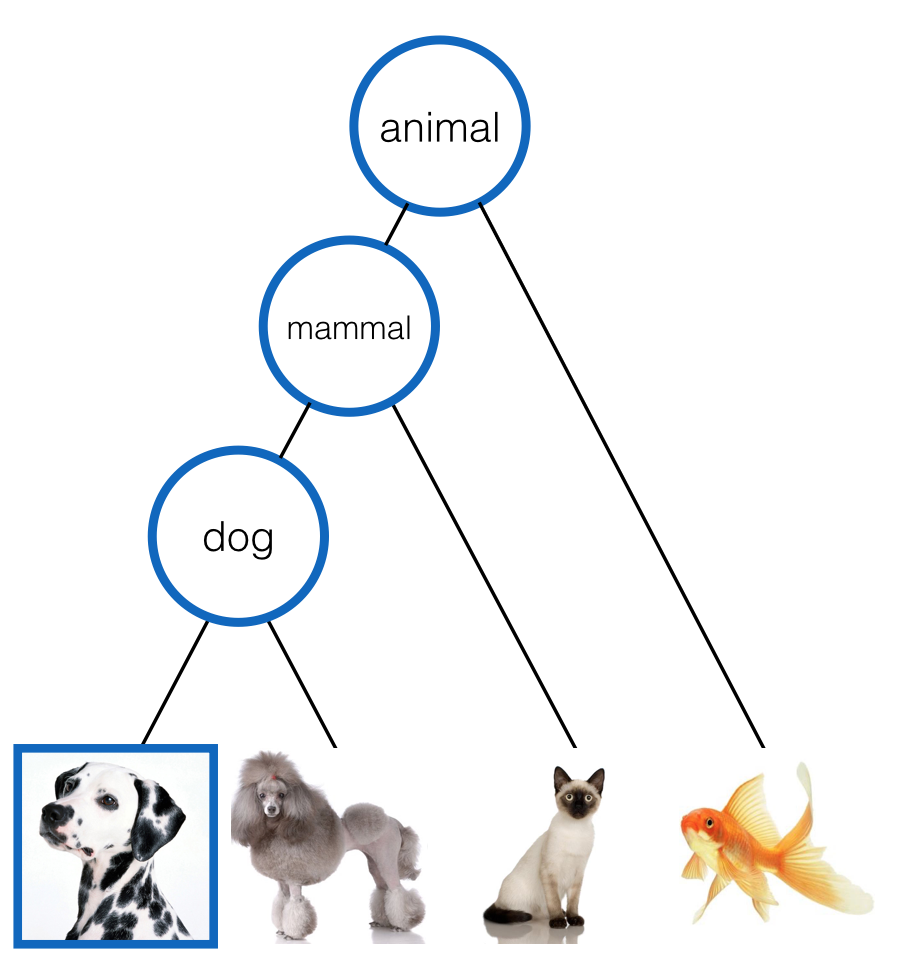
\includegraphics[scale = .2]{taskhierarchy}
\end{center}
\caption{Hierarchy of objects used in experiment 1}
\label{fig:taskhierarchy}
\end{figure}

\section{Experiment 1: \\ Questions and answers in a hierarchical world}

In order to test how questioners choose questions when given a decision problem, and how answerers choose answers under uncertainty about this decision problem, we designed a guessing-game task played by two players: a guesser and a helper. In this game, $4$ animals (a dalmatian, a poodle, a siamese cat, and a goldfish) were hidden behind $4$ gates. Note that these animals were arranged in a class hierarchy (see Fig. \ref{fig:taskhierarchy}). The guesser was given a private goal of finding one of the objects, and the helper had privileged information about the exact locations of each object. Before choosing a gate, the guesser could ask the helper a single question, and the helper could respond to this question by revealing the object behind a single gate. 

In terms of our model specification, the world space $\mathcal{W}$ is the set of $4! = 24$ possible assignments of four objects to four gates and the goal space $\mathcal{G}$ is the set of four objects that the guesser could possibly be trying to find, and the answer space $\mathcal{A}$ is the set of four gates that the helper could possibly reveal. The key constraint in the task, however, is that the guesser must choose from a \emph{restricted set of questions}: they may be trying to find the goldfish, but cannot directly ask `where is the goldfish?' Instead, the question space $\mathcal{Q}$ is the set of highlighted nodes in the hierarchy, including higher order nodes that are consistent with multiple answers. 
\begin{figure*}[t!]
\begin{center}
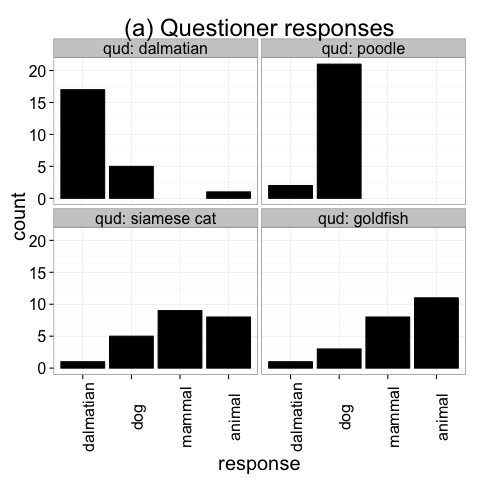
\includegraphics[scale = .5]{exp3_q}
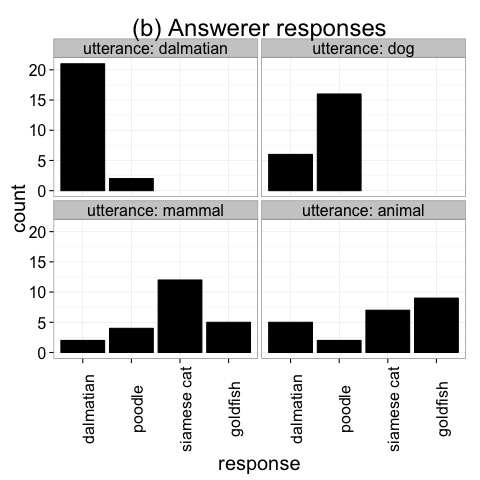
\includegraphics[scale = .5]{exp3_ans}
\end{center}
\caption{Experiment 1 results}
\label{fig:exp1res}
\end{figure*}
%\label{sec:expq}

We recruited 25 participants from Amazon Mechanical Turk to participate in this task. Each participant provided responses for four trials in the role of the questioner (corresponding to each goal in $\mathcal{G}$), and four trials in the role of the answerer (corresponding to each question in $\mathcal{Q}$). In order to collect responses for all elements of $\mathcal{G}$ and $\mathcal{Q}$, The order of� the questioner and answerer blocks was randomly assigned, and the order of stimuli within these blocks was also randomized\footnote{All materials are available on \href{https://github.com/hawkrobe/Q\_and\_A/tree/master/experiment3/versions/experiment3\_short}{Github}}. Two participants were excluded due to self-reported confusion about the task.

Results for the guesser role are shown in Figure \ref{fig:exp1res}(a). There are two primary trends to note in these data. First, questioners tend to choose the indirect question node closest to their goal when the direct question is unavailable. It is unsurprising that they ask about the `dalmatian` when looking for the dalmatian, but interesting that they strongly prefer asking about a `dog' when looking for the poodle, about a `mammal' when looking for the cat, and so on. \red{XXX Robert: need statistics here. Probably will need more than 25 participants to get enough power...} 


Results for the helper role are shown in Figure \ref{fig:exp1res}(b). The most striking feature of these data is how closely match the questioner distribution \red{XXX Robert: Possibly just because people did both... It might be the second-timers driving the effect, so we should separate out the different orders, or run it again between-subjects}. If the helper is asked about a `dog`, the dalmatian and poodle would be equally good literal answers to this question, but they strongly prefer to give the location of the poodle. Similarly, the dalmatian, poodle, and siamese cat are all mammals, but helpers prefer to respond to the `mammal' question by revealing the location of the cat. 



We will delay our full model evaluation until after describing a second experiment, but we suggest at this stage that some pragmatic inference appears be taking place on the part of the answerer. In discerning why the questioner would ask about the dog, they might reason as follows: `if the questioner wanted to know the location of the dalmatian, he or she would have asked about the dalmatian. They didn't, therefore, they must be interested in the other dog: the poodle.' 

To address concerns that the preceding results were due to particular features of the design such as the one-to-one mapping from goals to questions and from questions to answers, which gives the task the sense of an 'elimination game,' we ran a second experiment using a larger hierarchy \dots

\section{Experiment 2: }
\label{sec:expa}




\section{Model evaluation}
\label{sec:evaluation}



\begin{figure*}[t!]
\begin{center}
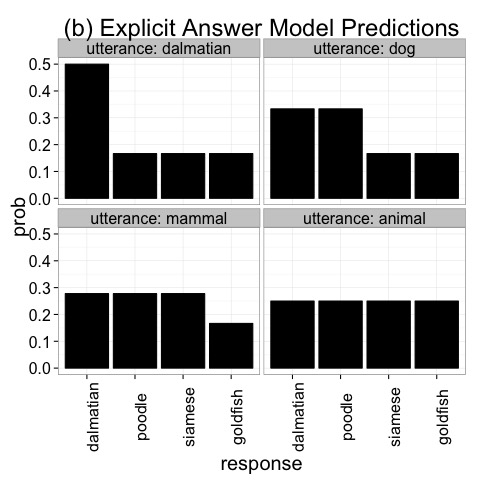
\includegraphics[scale = .5]{Exp3ExplicitAnswerPrediction}
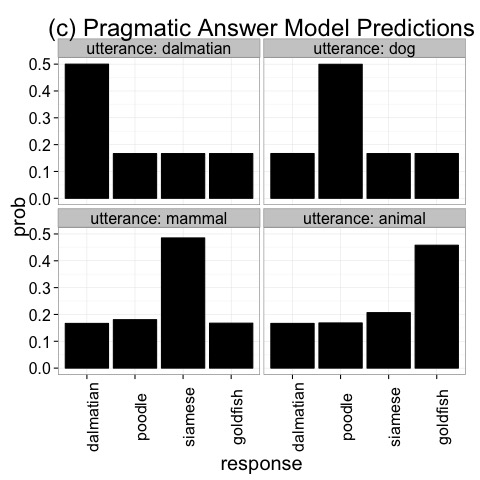
\includegraphics[scale = .5]{Exp3PragmaticAnswerPrediction}
\end{center}
\caption{Experiment 1 model predictions}
\label{fig:exp1pred}
\end{figure*}

\red{XXX}



\section{General discussion}
\label{sec:gd}

 In this paper we have presented evidence that question and answer behavior, a particular kind of action, also depends critically on participants signaling and inferring intentions. 

Behind every question lies some goal or intention. This could be an intention to obtain an explicit piece of information (``Where can I get a newspaper?''), signal some common ground (``Did you see the game last night?''), test the answerer's knowledge (``If I add these numbers together, what do I get?''), politely request the audience to take some action (``Could you pass the salt?''), or just to make open-ended small talk (``How was your weekend?''). Intuitively, different intentions seem to warrant different kinds of answers, even if the question is expressed using the same words. Viewing these questions as signals provides a new theoretical framework to analyze particular kinds of questions.

\red{XXX}

\bibliographystyle{apacite}

\setlength{\bibleftmargin}{.125in}
\setlength{\bibindent}{-\bibleftmargin}

\bibliography{bibs}


\end{document}
